\documentclass{article}
\usepackage{etoolbox}
\usepackage{tikz}
\usepackage{alphalph}
\usepackage{nicefrac}
\usetikzlibrary{external,shapes,calc,math,patterns,arrows,positioning,fadings}
\tikzexternalize[optimize=false]

\tikzstyle{node}=[circle, draw=black, minimum size=25pt, line width=1, inner sep= 5pt]
\tikzstyle{nodel}=[circle, draw=black, minimum size=15pt, line width=1, inner sep= 0pt]
\tikzstyle{nodem}=[circle, draw=black, minimum size=10pt, line width=1, inner sep= 0pt]
\tikzstyle{tnode}=[nodel, minimum size=0.8 cm, fill=white]
\tikzstyle{node1}=[circle, draw=black, minimum size=20pt, line width=1, inner sep= 2pt]
\tikzstyle{node2}=[circle, draw=black, minimum size=14pt, line width=1, inner sep= 0pt, fill=white!70!black]
\tikzstyle{l1}=[line width=1]
\tikzfading[name=fade right, left color=transparent!0, right color=transparent!100]
\tikzstyle{odd}=[node2, dashed, pattern=dots, pattern color=mred!75!white]
\tikzstyle{even}=[node2, pattern=dots, pattern color=mblue!75!white]
\tikzstyle{lodd}=[odd, pattern = crosshatch dots]
\tikzstyle{leven}=[even, pattern = crosshatch dots]
\tikzstyle{enset}=[node1, thick, double, font=\footnotesize]
\tikzstyle{onset}=[node1, thick, densely dashed, double, font=\footnotesize]
\tikzstyle{subtree}=[node1, opacity=0.3,dotted, font=\footnotesize]
\tikzstyle{undef}=[node1, dotted, pattern=dots, pattern color=black!25!white]
\tikzstyle{edge}=[above,midway,font=\tiny]
\tikzstyle{smallarrow} = [draw, single arrow, shape border rotate=270, minimum height=0.25cm, minimum width=0.35cm, single arrow head extend=0.01cm, inner sep=0]

\newcommand\DLINE[4]{
  \draw (#1, #2) ++ (-.3,-.9) node[inner sep=0] (lb) {} ++(#3,0) ++(.6,0) node[inner sep=0] (rb) {} ++(0,0.4) node[inner sep=0] (rt) {};;
  \path[fill=white!80!black, rounded corners=2pt] (lb) rectangle (rt);
  \ifnumequal{#4}{1}{\draw[thin] (lb) -- (rb);}{}
}

\usepackage{xcolor}
\definecolor{mblue}{HTML}{1F77B4}
\definecolor{morange}{HTML}{FF7F0E}
\definecolor{mgreen}{HTML}{2CA02C}
\definecolor{mred}{HTML}{D62728}
\definecolor{mpurple}{HTML}{9467BD}
\definecolor{mbrown}{HTML}{8C564B}
\definecolor{mpink}{HTML}{E377C2}
\definecolor{mgrey}{HTML}{7F7F7F}
\definecolor{mlime}{HTML}{BCBD22}
\definecolor{mcyan}{HTML}{17BECF}

% Set new commands
\newcommand{\codeword}[1]{\texttt{\textcolor{MidnightBlue}{#1}}}
%\newcommand{\codefunc}[1]{\texttt{\textcolor{OliveGreen}{#1}}}
\let\oldemptyset\emptyset
\let\emptyset\varnothing
\newcommand{\codefunc}[1]{\texttt{#1}}
\newcommand{\m}[1]{\mathcal{#1}}
\newcommand{\n}[1]{\mathscr{#1}}
\newcommand{\bound}{\mathscr{B}}
\newcommand{\akker}{\mathscr{A}}
\newcommand{\nset}{\mathcal{N}}
\newcommand{\vset}{\mathcal{V}}
\newcommand{\pre}[1]{ {}^{#1} }
\newcommand{\ceil}[1]{{\left \lceil #1 \right \rceil }}
\newcommand{\floor}[1]{{\left \lfloor #1 \right \rfloor }}


\begin{document}

% PMW
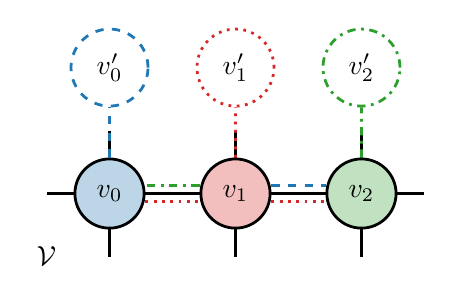
\begin{tikzpicture}[scale=0.8]
    \node at (-1, -1) {$\mathcal{V}$};
    \draw[l1] (0, 0) -- (4,0);
    \draw[l1] (-1,0) -- (5,0);
    \draw[l1] (0,1) -- (0,-1);
    \draw[l1] (2,1) -- (2,-1);
    \draw[l1] (4,1) -- (4,-1);
    \node[node, fill=white!70!mblue, text opacity=1] at (0,0) (1) {$v_0$};
    \node[node, draw=mblue, dashed] at (0,2) (2) {$v_0'$};
    \node[node, fill=white!70!mred, text opacity=1] at (2,0) (3){$v_1$};
    \node[node, draw=mred,dotted] at (2,2) (4) {$v_1'$};
    \node[node, fill=white!70!mgreen, text opacity=1] at (4,0) (5) {$v_2$};
    \node[node, draw=mgreen, dashdotted] at (4,2) (6) {$v_2'$};

    \draw[l1, dashed, mblue] (1) -- (2);
    \draw[l1, dashed, mblue, transform canvas={yshift=3pt}] (3) -- (5);
    \draw[l1, dotted, mred] (3) -- (4);
    \draw[l1, dotted, mred, transform canvas={yshift=-3pt}] (1) -- (3) -- (5);
    \draw[l1, dashdotted, mgreen] (5) -- (6);
    \draw[l1, dashdotted, mgreen, transform canvas={yshift=3pt}] (3) -- (1);
\end{tikzpicture}


% Node-tree
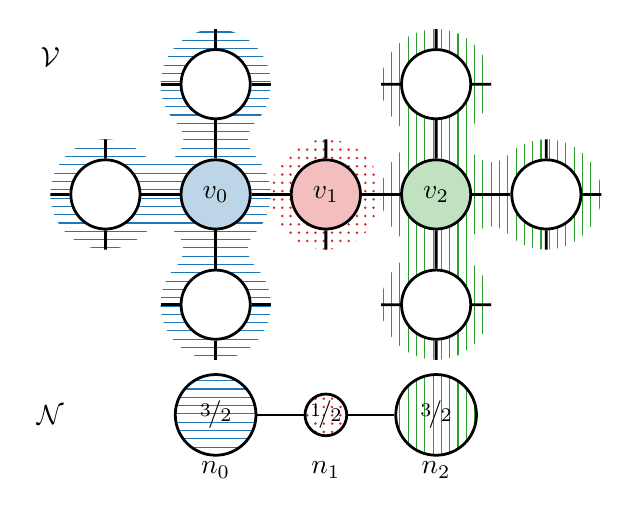
\begin{tikzpicture}[scale=0.7]
    \path[pattern=horizontal lines, pattern color=mblue] (0,3) arc (90:225:1) arc (45:-135:.4142) arc (45:315:1) arc (135:-45:.4142) arc (135:405:1) arc (225:135:.4142) arc (-45:45:1) arc (225:135:.4142) arc (-45:90:1) -- cycle;

    \begin{scope}[shift={(4,0)}, xscale=-1]
        \path[pattern=vertical lines, pattern color=mgreen] (0,3) arc (90:225:1) arc (45:-135:.4142) arc (45:315:1) arc (135:-45:.4142) arc (135:405:1) arc (225:135:.4142) arc (-45:45:1) arc (225:135:.4142) arc (-45:90:1) -- cycle;
    \end{scope}
    \path[pattern=dots , pattern color=mred] (2,1) arc (90:450:1);

    \node[node, fill=white!70!mblue] at (0,0) (0) {$v_0$};
    \node[node, fill=white!70!mred] at (2,0) (1) {$v_1$};
    \node[node, fill=white!70!mgreen] at (4,0) (5) {$v_2$};
    \node[node, fill=white] at (-2,0) (2) {};
    \node[node, fill=white] at (0,2) (3) {};
    \node[node, fill=white] at (0,-2) (4) {};
    \node[node, fill=white] at (6,0) (6) {};
    \node[node, fill=white] at (4,2) (7) {};
    \node[node, fill=white] at (4,-2) (8) {};

    \draw[l1] (2) -- +(-1,0) (2) -- +(0,1) (2) -- +(0,-1);
    \draw[l1] (3) -- +(1,0) (3) -- +(-1,0) (3) -- +(0,1);
    \draw[l1] (4) -- +(1,0) (4) -- +(-1,0) (4) -- +(0,-1);
    \draw[l1] (6) -- +(1,0) (6) -- +(0,1) (6) -- +(0,-1);
    \draw[l1] (7) -- +(1,0) (7) -- +(-1,0) (7) -- +(0,1);
    \draw[l1] (8) -- +(1,0) (8) -- +(-1,0) (8) -- +(0,-1);


    \draw[l1] (6) -- (5) -- (1) -- (0) -- (3);
    \draw[l1] (2) -- (0) -- (4);
    \draw[l1] (7) -- (5) -- (8);
    \draw[l1] (2, 1) -- (1) -- (2,-1);
    \node at (-3, 2.5) {$\mathcal{V}$};

    \begin{scope}[shift={(0, -4)}]
        \node at (-3, 0) {$\mathcal{N}$}; 
        \node[node, pattern=horizontal lines, pattern color=mblue] at (0,0) (d) {$\nicefrac{3}{2}$};
        \node[nodel, pattern=dots , pattern color=mred] at (2,0) (e) {$\nicefrac{1}{2}$};
        \node[node, pattern=vertical lines, pattern color=mgreen] at (4,0) (f) {$\nicefrac{3}{2}$};
        \node at (0,-1) {$n_0$};
        \node at (2,-1) {$n_1$};
        \node at (4,-1) {$n_2$};
        \draw[l1] (d) -- (e) -- (f);
    \end{scope}
\end{tikzpicture}


% Node types
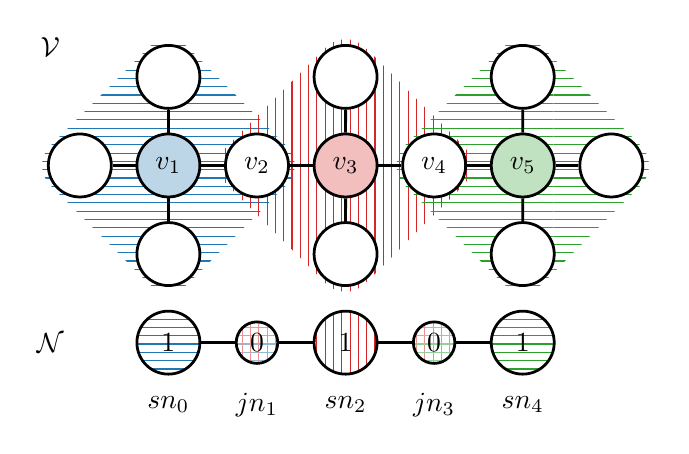
\begin{tikzpicture}[scale=0.75]
    \node at (-3, 2) {$\mathcal{V}$};
    \node at (-3, -3) {$\mathcal{N}$}; 
    \begin{scope}[shift={(-1, 0)}, scale=1.5]
        \node at (0,0) (0) {}; \node at (2,0) (1) {}; \node at (4,0) (2) {};        
        \path[pattern=horizontal lines, pattern color=mblue, rounded corners=10pt, rotate around={45:(0)}] (-1.1,-1.1) rectangle (1.1,1.1);
        \path[pattern=vertical lines, pattern color=mred, rounded corners=10pt, rotate around={45:(1)}] (0.9,-1.1) rectangle (3.1,1.1);
        \path[pattern=horizontal lines, pattern color=mgreen, rounded corners=10pt, rotate around={45:(2)}] (2.9,-1.1) rectangle (5.1,1.1);
    
        \node[tnode, fill=white!70!mblue] at (0) (v0) {$v_1$};
        \node[tnode] at (-1,0) (v0l) {};
        \node[tnode] at (0,1) (v0u) {};
        \node[tnode] at (0,-1) (v0d) {};
    
        \node[tnode, fill=white!70!mred] at (1) (v1) {$v_3$};
        \node[tnode] at (1,0) (v1l) {$v_{2}$};
        \node[tnode] at (2,1) (v1u) {};
        \node[tnode] at (2,-1) (v1d) {};
    
        \node[tnode, fill=white!70!mgreen] at (2) (v2) {$v_5$};
        \node[tnode] at (3,0) (v2l) {$v_{4}$};
        \node[tnode] at (5,0) (v2r) {};
        \node[tnode] at (4,1) (v2u) {};
        \node[tnode] at (4,-1) (v2d) {};
    
        \draw[l1] (v0l) -- (v0) -- (v1l) -- (v1) -- (v2l) -- (v2) -- (v2r);
        \draw[l1] (v0u) -- (v0) -- (v0d);
        \draw[l1] (v1u) -- (v1) -- (v1d);
        \draw[l1] (v2u) -- (v2) -- (v2d);
    \end{scope}

    \begin{scope}[shift={(-1, -3)}, scale=1.5]
        \node[tnode, pattern=horizontal lines, pattern color=mblue] at (0,0) (n0) {1};
        \node[nodel, pattern=horizontal lines, pattern color=mblue!50!white, line width=0] at (1,0) {};
        \node[nodel, pattern=vertical lines,   pattern color=mred!50!white] at (1,0) (j01) {0};
        \node[tnode, pattern=vertical lines , pattern color=mred] at (2,0) (n1) {1};
        \node[nodel, pattern=vertical lines,   pattern color=mred!50!white, line width=0] at (3,0) {};
        \node[nodel, pattern=horizontal lines, pattern color=mgreen!50!white] at (3,0) (j12) {0};
        \node[tnode, pattern=horizontal lines, pattern color=mgreen] at (4,0) (n2) {1};
        \node at (0,-.7) {$sn_0$};
        \node at (1,-.7) {$jn_{1}$};
        \node at (2,-.7) {$sn_2$};
        \node at (3,-.7) {$jn_{3}$};
        \node at (4,-.7) {$sn_4$};
        \draw[l1] (n0) -- (j01) -- (n1) -- (j12) -- (n2);
    \end{scope}
\end{tikzpicture}

% DFS
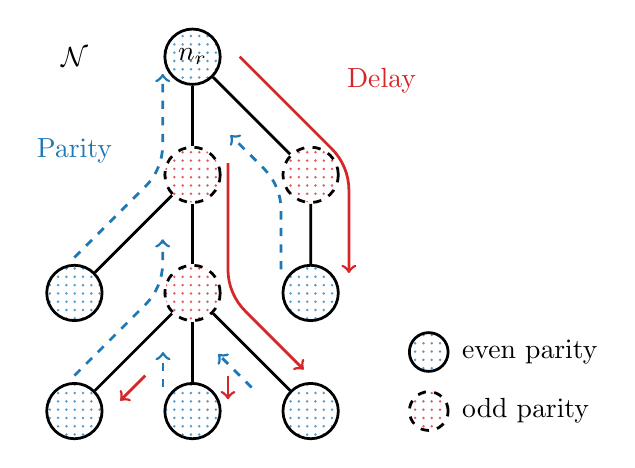
\begin{tikzpicture}[x=1.5cm,y=1.5cm]
    \node[even,node1] (a) at (1, 3) {$n_r$};
    \node[odd ,node1]  (b) at (1, 2) {};
    \node[odd ,node1]  (c) at (1, 1) {};
    \node[even,node1] (d) at (1, 0) {};
    \node[even,node1] (e) at (0, 1) {};
    \node[even,node1] (f) at (0, 0) {};
    \node[odd ,node1]  (g) at (2, 2) {};
    \node[even,node1] (h) at (2, 1) {};
    \node[even,node1] (i) at (2, 0) {};
    \draw[l1] (a) -- (b) -- (c) -- (d);
    \draw[l1] (b) -- (e);
    \draw[l1] (c) -- (f);
    \draw[l1] (c) -- (i);
    \draw[l1] (a) -- (g) -- (h);

    \draw[l1, ->, dashed, color=mblue] (0, 1.3) -- +(45:0.85) arc (-45:0:.5) -- +(90:.6);
    \draw[l1, ->, dashed, color=mblue] (0, 0.3) -- +(45:0.85) arc (-45:0:.5) -- +(90:.2);
    \draw[l1, ->, dashed, color=mblue] (0.75,0.2) -- +(90:.3);
    \draw[l1, ->, dashed, color=mblue] (1.5,0.2) -- +(135:.4);
    \draw[l1, ->, dashed, color=mblue] (1.75,1.2) -- +(90:0.5) arc (0:45:.5) -- +(135:0.4);
    \draw[l1, ->, color=mred] (1.4, 3) -- +(-45:1.1) arc (45:0:0.5) -- +(-90:0.7);
    \draw[l1, ->, color=mred] (1.3, 2.1) -- +(-90:0.9) arc (180:225:.5) -- +(-45:0.7);
    \draw[l1, ->, color=mred] (0.6, 0.3) -- +(225:.3);
    \draw[l1, ->, color=mred] (1.3, 0.3) -- +(-90:.2);
    \node[text=mblue] at (0,2.2) {Parity};
    \node[text=mred] at (2.6,2.8) {Delay};
    \node at (0,3) {$\mathcal{N}$};

    \path (3,.5) node[node1, even]{} -- +(.2,0) node[anchor=west] {even parity}; 
    \path (3,0) node[node1, odd]{} -- +(.2,0) node[anchor=west] {odd parity}; 
\end{tikzpicture}



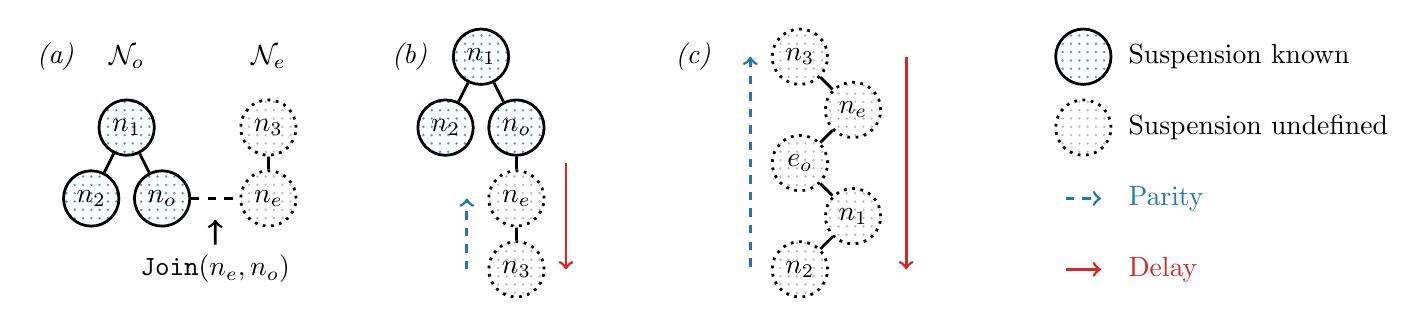
\begin{tikzpicture}[scale=0.9]
    \node at (1.5,2) {$\nset_o$};
    \node at (3.5,2) {$\nset_e$};
    \node (o1) [even, node1] at (1.5, 1) {$n_1$};
    \node (o2) [even, node1] at (1, 0) {$n_2$};
    \node (o3) [even, node1] at (2, 0) {$n_o$};
    \node (e4) [undef] at (3.5,1) {$n_3$};
    \node (e5) [undef] at (3.5,0) {$n_e$};
    \draw[l1] (o2) -- (o1) -- (o3) (e4) -- (e5);
    \draw[l1, dashed] (o3) -- (e5) node[midway,below] (a) {};
    \draw[l1, <-] (a) -- ++(0,-.5) node[below] {$\codefunc{Join}(n_e, n_o)$};
  
    \begin{scope}[shift={(5,1)}]
    \node (o1) [even, node1] at (1.5, 1) {$n_1$};
    \node (o2) [even, node1] at (1, 0) {$n_2$};
    \node (o3) [even, node1] at (2, 0) {$n_o$};
    \node (e4) [undef] at (2,-2) {$n_3$};
    \node (e5) [undef] at (2,-1) {$n_e$};
    \draw[l1] (o2) -- (o1) -- (o3) -- (e5) -- (e4);
    \draw[l1, ->, dashed, color=mblue] (e4) ++(-.7,0) -- + (0,1);
    \draw[l1, ->, color=mred] (o3) ++(.7,-.5) -- +(0,-1.5);
    \end{scope}
  
    \begin{scope}[shift={(11,-1)}]
    \node (o1) [undef] at (0.75, 0.75) {$n_1$};
    \node (o2) [undef] at (0, 0) {$n_2$};
    \node (o3) [undef] at (0, 1.5) {$e_o$};
    \node (e4) [undef] at (0,3) {$n_3$};
    \node (e5) [undef] at (0.75,2.25) {$n_e$};
    \draw[l1] (o2) -- (o1) -- (o3) -- (e5) -- (e4);
    \draw[l1, <-, dashed, color=mblue] (e4) ++(-.7,0) -- +(0,-3);
    \draw[l1, ->, color=mred] (e4) ++(1.5,0) -- +(0,-3);
    \end{scope}
  
    \node at (0.5,2) {\emph{(a)}};
    \node at (5.5,2) {\emph{(b)}};
    \node at (9.5,2) {\emph{(c)}};

    \begin{scope}[shift={(15,0)}]
        \path (0, 2) node[even, node1] {} -- +(.5,0) node[anchor=west]{Suspension known};
        \path (0, 1) node[undef] {} -- +(.5,0) node[anchor=west]{Suspension undefined};
        \draw[l1, ->, color=mred] (-.25, -1) -- ++(0.5,0);
        \node[color=mred, anchor=west] at (.5,-1) {Delay};
        \draw[l1, ->, color=mblue, dashed] (-.25, 0) -- ++(0.5,0);
        \node[color=mblue, anchor=west] at (.5,0) {Parity};
    \end{scope}

\end{tikzpicture}

% Equilibrium

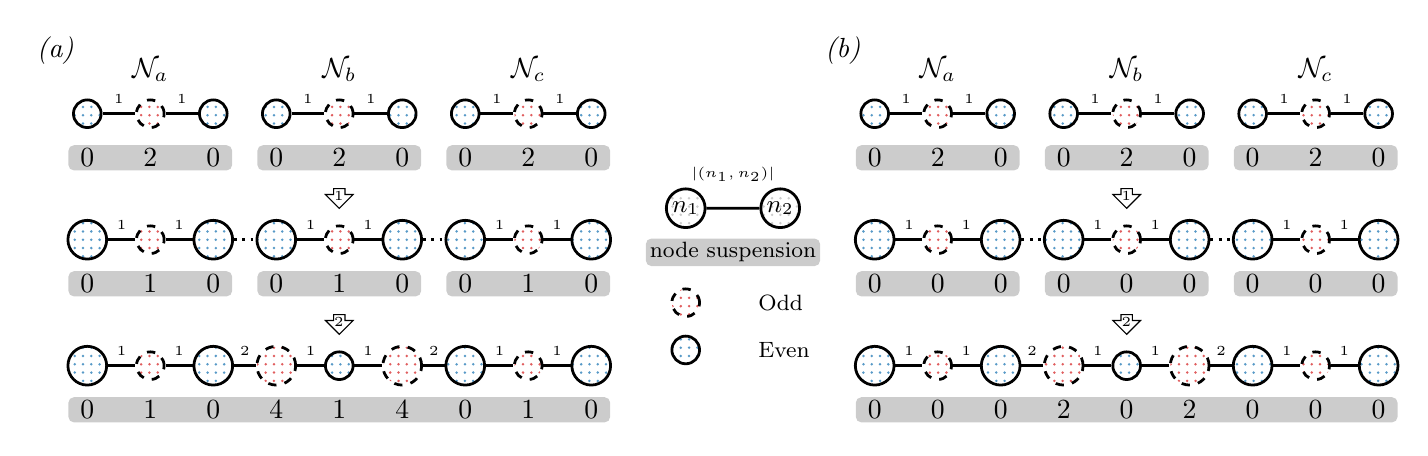
\begin{tikzpicture}[on grid, scale=0.8]

    \begin{scope}[shift={(9.5,-3.5)}]
        \node[node2, pattern=dots, pattern color=black!20!white] (n1) at (0,2) {\small$n_1$}; 
        \node[node2, pattern=dots, pattern color=black!20!white] (n2) at (1.5,2) {\small$n_2$}; 
        \draw[l1] (n1) -- (n2) node[edge, above=0.2cm]{$|(n_1, n_2)|$};
        \node[align=center, fill=white!80!black, rounded corners=2pt, inner sep=0.5mm] at (0.75, 1.3) {\footnotesize node suspension};
        \draw (0, 0.5) node[odd, nodem]{} +(1,0) node[align=left, anchor=west]{\footnotesize Odd };
        \draw (0, -0.25) node[even, nodem]{} +(1,0) node[align=left, anchor=west]{\footnotesize Even };
    \end{scope}

    \node at (-.5,1) {\emph{(a)}};
    \node[smallarrow, label={[label distance=-3.6mm]0:\tiny 1}] at (4, -1.3) {};

    \foreach \x in {0,3,6}{\DLINE{\x}{0}{2}{0}}
      \foreach \x in {0,2,3,5,6,8}{\draw (\x,0) node [even, nodem] (a\x) {} ++(0,-.7) node (ad\x) {0};}
      \foreach[count=\i] \x in {1,4,7}{      \draw (\x,0) node [odd, nodem]  (a\x) {} ++(0,-.7) node (ad\x) {2};
                                             \node at (\x,0.7) {$\nset_{\alphalph{\i}}$};}
      \draw[l1] (a0) -- (a1) node[edge]{1} -- (a2) node[edge]{1} (a3) -- (a4) node[edge]{1} -- (a5) node[edge]{1} (a6) -- (a7) node[edge]{1} -- (a8) node[edge]{1};

    \begin{scope}[shift={(0,-2)}]
        \node[smallarrow, label={[label distance=-3.6mm]0:\tiny 2}] at (4, -1.3) {};
        \foreach \x in {0,3,6}{\DLINE{\x}{0}{2}{0}}
        \foreach \x in {0,2,3,5,6,8}{\draw (\x,0) node [even] (e\x) {} ++(0,-.7) node {0};}
        \foreach \x in {1,4,7}{      \draw (\x,0) node [odd, nodem]  (e\x) {} ++(0,-.7) node {1};}
        \draw[l1] (e0) -- (e1) node[edge]{1} -- (e2) node[edge]{1} (e3) -- (e4) node[edge]{1} -- (e5) node[edge]{1} (e6) -- (e7) node[edge]{1} -- (e8) node[edge]{1};
        \draw[l1, dotted] (e2) -- (e3) (e5) -- (e6);
    \end{scope}

    \begin{scope}[shift={(0,-4)}]
        \DLINE{0}{0}{8}{0}
        \foreach \x in {0,2,6,8}{\draw (\x,0) node [even] (b\x) {} ++(0,-.7) node {0};}
        \foreach \x in {1,7}{    \draw (\x,0) node [odd, nodem]  (b\x) {} ++(0,-.7) node {1};}
        \foreach \x in {3,5}{    \draw (\x,0) node [odd]  (b\x) {} ++(0,-.7) node {4};}
                                 \draw (4,0)  node [even, nodem] (b4)  {} ++(0,-.7) node {1};
        \draw[l1] (b0) -- (b1) node[edge]{1} -- (b2) node[edge]{1} -- (b3) node[edge]{2} -- (b4) node[edge]{1} -- (b5) node[edge]{1} -- (b6) node[edge]{2} -- (b7) node[edge]{1} -- (b8) node[edge]{1};
    \end{scope}

        
    \begin{scope}[shift={(12.5,0)}]
        \node at (-.5,1) {\emph{(b)}};
        \node[smallarrow, label={[label distance=-3.6mm]0:\tiny 1}] at (4, -1.3) {};

        \foreach \x in {0,3,6}{\DLINE{\x}{0}{2}{0}}
        \foreach \x in {0,2,3,5,6,8}{\draw (\x,0) node [even, nodem] (c\x) {} ++(0,-.7) node {0};}
        \foreach[count=\i] \x in {1,4,7}{      \draw (\x,0) node [odd, nodem]  (c\x) {} ++(0,-.7) node (cd\x) {2};
                                               \node at (\x,0.7) {$\nset_{\alphalph{\i}}$};}
        \draw[l1] (c0) -- (c1) node[edge]{1} -- (c2) node[edge]{1} (c3) -- (c4) node[edge]{1} -- (c5) node[edge]{1} (c6) -- (c7) node[edge]{1} -- (c8) node[edge]{1};
  
        \begin{scope}[shift={(0,-2)}]
            \node[smallarrow, label={[label distance=-3.6mm]0:\tiny 2}] at (4, -1.3) {};
            \foreach \x in {0,3,6}{\DLINE{\x}{0}{2}{0}}
            \foreach \x in {0,2,3,5,6,8}{\draw (\x,0) node [even] (c\x) {} ++(0,-.7) node {0};}
            \foreach \x in {1,4,7}{      \draw (\x,0) node [odd, nodem]  (c\x) {} ++(0,-.7) node {0};}
            \draw[l1] (c0) -- (c1) node[edge]{1} -- (c2) node[edge]{1} (c3) -- (c4) node[edge]{1} -- (c5) node[edge]{1} (c6) -- (c7) node[edge]{1} -- (c8) node[edge]{1};
            \draw[l1, dotted] (c2) -- (c3) (c5) -- (c6);
        \end{scope}
  
        \begin{scope}[shift={(0,-4)}]
            \DLINE{0}{0}{8}{0}
            \foreach \x in {0,2,6,8}{\draw (\x,0) node [even] (d\x) {} ++(0,-.7) node {0};}
            \foreach \x in {1,7}{    \draw (\x,0) node [odd, nodem]  (d\x) {} ++(0,-.7) node {0};}
            \foreach \x in {3,5}{    \draw (\x,0) node [odd]  (d\x) {} ++(0,-.7) node {2};}
                                    \draw (4,0)  node [even, nodem] (d4)  {} ++(0,-.7) node {0};
            \draw[l1] (d0) -- (d1) node[edge]{1} -- (d2) node[edge]{1} -- (d3) node[edge]{2} -- (d4) node[edge]{1} -- (d5) node[edge]{1} -- (d6) node[edge]{2} -- (d7) node[edge]{1} -- (d8) node[edge]{1};
        \end{scope}
    \end{scope}
\end{tikzpicture}

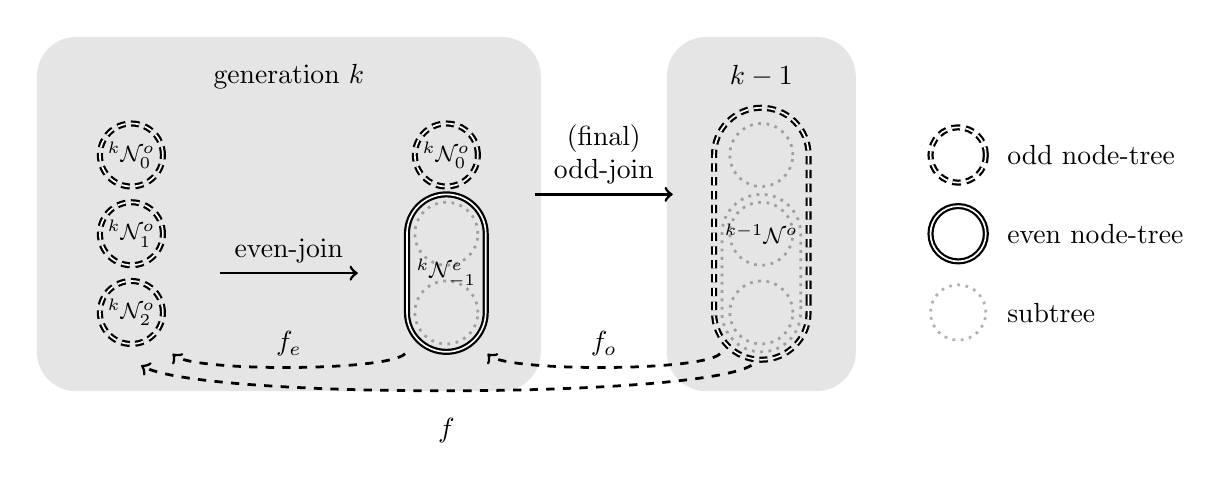
\begin{tikzpicture}[node distance=1cm, on grid]

    \node (a) at (0,0) {};
    \node (b) [right = 4cm of a] {};
    \node (c) [right = 4cm of b] {};
    \node (d) [right = 3cm of c] {};

    \node (b1l) [below left = 1cm and 1.2cm of a] {};
    \node (b1r) [above right = 3.5cm and 1.2cm of b] {};
    \path[fill=black!10!white, rounded corners=0.5cm] (b1l) rectangle (b1r);
    \node (b1t) at ($(a)!0.5!(b)$) {}; \node [above=3cm of b1t] {generation $k$};
    \node (b2l) [below left = 1cm and 1.2cm of c] {};
    \node (b2r) [above right = 3.5cm and 1.2cm of c] {};
    \path[fill=black!10!white, rounded corners=0.5cm] (b2l) rectangle (b2r);
    \node [above=3cm of c] {$k-1$};

    \begin{scope}[shift={(10.5,0)}]
      \path (0,2) node[onset]{} -- +(.5,0)node[anchor=west]{odd node-tree};
      \path (0,1) node[enset]{} -- +(.5,0)node[anchor=west]{even node-tree};
      \path (0,0) node[subtree]{} -- +(.5,0)node[anchor=west]{subtree};
    \end{scope}

    \node (a0) [above = 0 cm of a] {\footnotesize $\pre{k}\mathcal{N}^o_2$};
    \node (a1) [above = 1 cm of a] {\footnotesize $\pre{k}\mathcal{N}^o_1$};
    \node (a2) [above = 2 cm of a] {\footnotesize $\pre{k}\mathcal{N}^o_0$};
    \draw[onset] (a0) circle[radius=.4cm];
    \draw[onset] (a1) circle[radius=.4cm];
    \draw[onset] (a2) circle[radius=.4cm];

    \foreach \i in {0,1,2}{
        \node (b\i) [above = \i cm of b] {};
    }
    \node at (b2) {\footnotesize $\pre{k}\mathcal{N}^o_0$};
    \node at ($(b0)!0.5!(b1)$) {\footnotesize $\pre{k}\mathcal{N}^e_{-1}$};
    \draw[onset] (b2) circle[radius=0.4cm];
    \draw[subtree] (b1) circle[radius=.4cm];
    \draw[subtree] (b0) circle[radius=.4cm];
    \node[right = 0.5cm of b] (bc) {};
    \draw[enset] (bc) -- +(0, 1) arc (0:180:0.5) -- +(0, -1) arc (180:360:0.5) -- cycle;

    \foreach \i in {0,1,2}{
      \node (c\i) [above =\i cm of c] {};
      \draw[subtree] (c\i) circle[radius=.4cm];
    }
    \node[right = 0.5cm of c] (cc1) {}; \node[right = 0.6cm of c] (cc2) {};
    \draw[subtree] (cc1) -- +(0, 1) arc (0:180:0.5) -- +(0, -1) arc (180:360:0.5) -- cycle;
    \draw[onset] (cc2) -- +(0, 2) arc (0:180:0.6) -- +(0, -2) arc (180:360:0.6) -- cycle;
    \node at (c1) {\footnotesize $\pre{k-1}\mathcal{N}^o$};

    \node (f1a) [below left = 0.4cm and 0.4cm of c] {}; \node (f1b) [below right = 0.4cm and 0.4cm of b] {};
    \node (f2a) [below left = 0.4cm and 0.4cm of b] {}; \node (f2b) [below right = 0.4cm and 0.4cm of a] {};
    \node (fa) [below = 0.6cm of c] {}; \node (fb) [below = 0.6cm of a] {};
    \draw[l1, ->, dashed] (f1a) .. controls +(225:0.5cm) and +(315:0.5cm) .. (f1b);
    \draw[l1, ->, dashed] (f2a) .. controls +(225:0.5cm) and +(315:0.5cm) .. (f2b);
    \draw[l1, ->, dashed] (fa)  .. controls +(210:1cm) and +(330:1cm) .. (fb);

    \node (ca) at ($(c)!0.5!(a)$) {}; \node [below = 1.5cm of ca] {$f$};
    \node (cb) at ($(c)!0.5!(b)$) {}; \node [below = 0.4cm of cb] {$f_o$};
    \node [below = 0.4cm of b1t] {$f_e$};

    \node (u1lt) at ($(a0)!0.5!(a1)$) {}; \node(u1l) [right=1cm of u1lt] {};
    \node (u1rt) at ($(b0)!0.5!(b1)$) {}; \node(u1r) [left=1cm of u1rt] {};
    \node (u2lt) at ($(b1)!0.5!(b2)$) {}; \node(u2l) [right=1cm of u2lt] {};
    \node (u2rt) at ($(c1)!0.5!(c2)$) {}; \node(u2r) [left=1cm of u2rt] {};
    \draw[l1, ->] (u1l) -- (u1r) node[midway,above] {even-join};
    \draw[l1, ->] (u2l) -- (u2r) node[midway,above, text width = 2cm, align=center] {(final)\\odd-join};

\end{tikzpicture}
\end{document}